\chapter{Results and Interpretation}
\label{cap7}

\textit{The results of the search of a high mass Higgs boson are presented. Signal and backgrounds templates are fitted to the data. No excesses beyond the SM expectations are found. Therefore, upper limits on signal production are computed in the form of 95\% CL exclusion limits on the production cross-section. These limits are also interpreted in term of 2HDM. I have done, in particular, the limits calculations for the 
fully-leptonic analysis and I have contributed to the combination among fully leptonic and semileptonic analysis. }

\section{Statistical interpretation}
\label{StatIn}
The Bayesian and the classical frequentist~\cite{cowan1998statistical}, with a number of modifications, are two statistical approaches commonly used in high energy physics for characterising the absence
of a signal.
Both methods allow one to quantify the level of incompatibility of data with a signal
hypothesis,  which  is  expressed  as  a  confidence  level  (C.L.)~\cite{CMS-NOTE-2011-005}. For excluding a signal the C.L. 95\% is a common choice.
The C.L. probabilistic interpretation is used when stating the non-existence
of a signal is not straightforward, as in the high mass analysis, and it is the subject of a vast body of literature.
The procedure used to calculate the upper limits is based on the frequentist approach using the likelihood ratio as test statistic. In addition to the parameter of interest such as the cross section of the signal, the signal and the background models contain several nuisance parameters whose values are not know n\textit{a priori}, but rather must be fitted on the data ~\cite{Cowan:2010js}.
In the following the frequentist approach is described.  The expected high mass signal  event yields will be generically denoted as $s$ and the backgrounds as $b$.
\newline
The most powerful statistic test to discriminate among different hypotheses, according to the Neyman-Pearson lemma~\cite{cowan1998statistical}, is the likelihoods ratio. In this case, where the two hypotheses differ for the presence of the signal in addition to the background, this ratio is  
\begin{equation}
  \lambda (\mu)=\frac{\mathcal{L}(data | \mu s +b)  }{ \mathcal{L}(data | b) }  \end{equation}
where, $\mathcal{L}$ is the likelihood function from the product of Poisson probabilities and  $\mu$ is the strength of the signal process (the case $\mu =0$ correspond to background only hypothesis, $\mu=1$ the the nominal signal hypothesis).
%One can see that $0 \leq  \lambda (\mu) \leq 1 $, $\mu$ near 1 is a evidence of good agreement among data and the hypothesized $\mu$ value.\\
It is convenient, for numerical reason, to use the test statistic $q_{\mu}$ defined as,  
\begin{equation}
 q_{\mu}= -2 \ln \lambda (\mu)  \end{equation}
where high value of $q_{\mu}$ correspond to low compatibility between data and the value of $\mu$. \\
Using the statistic test  $q_{\mu}$, is possible to quantify the level of disagreement between the data and the hypothesis using the $p$-value, defined as,
\begin{equation}
  p_{\mu}=  \int_{ q_{\mu},obs }^{\infty } f(q_{\mu}| \mu  ) dq_{\mu}   \end{equation}
where $ q_{\mu,obs} $ is the value of statistic test $q_{\mu}$ observed from the data and $f(q_{\mu}| \mu  )$ is the pdf of $q_{\mu}$ under the assumption of the signal strength $\mu$.
\newline
The systematic uncertainties on signal $s$ and background $b$ rates can be introduced as a dependence on some unknown set of nuisance parameters $\theta$. The test statistic then takes the following form:
\begin{equation}
 q_{\mu} =\frac{\mathcal{L}(data | \mu, \hat{\theta}_{\mu} )  }{ \mathcal{L}(data |0, \hat{\theta}_0 )},  \end{equation}
where $\hat{\theta}_{\mu}$ and $\hat{\theta}_0$ are the maximum likelihood estimators for the signal+background
hypothesis (with the signal strength factor $\mu$) and for the
background-only hypothesis ($\mu =0$). 
The profile likelihood test statistic is however modified to prevent negative signal values to
\begin{equation}
 \tilde{q}_{\mu} =\frac{\mathcal{L}(data | \mu, \hat{\theta}_{\mu} )  }{ \mathcal{L}(data |\hat{\mu}, \hat{\theta} )}, \; \; 0 \leq \hat{\mu} \leq \mu \; ,  \end{equation}
where $\hat{\mu}$ and $\hat{\theta}$ gives the global maximum of the likelihood. 
The constrain  $0 \leq \hat{\mu}$ is due to a positive signal rate, while the   $\hat{\mu} \leq \mu$ is imposed by hand in order to guarantee a one-sided  confidence interval.\\
At this point is useful to evaluate the observed statistic test $\tilde{q}_{\mu}^{obs}$ and the nuisance parameters $\hat{\theta}_0^{obs}$, $\hat{\theta}_{\mu}^{obs}$ that describe  the  experimentally observed data for the background-only and signal+background hypotheses, respectively.
With this in mind, the pdf of the test statistic is constructed by generating toy MC pseudo-data for both the background-only and signal+background hypotheses, 
$f(\tilde{q}_{\mu}| \mu, \hat{\theta}_{\mu}^{obs}  )$ and $f(\tilde{q}_{\mu}| \mu, \hat{\theta}_{0}^{obs}  )$. The corresponding $p$-value for the
signal+background and background-only hypotheses, $p_{\mu}$ and $p_b$ are given by:


\begin{equation}
  p_{\mu}= P( \tilde{q}_{\mu} \geq \tilde{q}_{\mu}^{obs} | signal+background)=  \int_{ q_{\mu},obs }^{\infty } f(\tilde{q}_{\mu}| \mu, \hat{\theta}_{\mu}^{obs}   ) d \tilde{q}_{\mu}   \end{equation}


\begin{equation}
 1- p_{b}= P( \tilde{q}_{\mu} \geq \tilde{q}_{\mu}^{obs} | background\mathrm{-}only)=  \int_{ q_{0},obs }^{\infty } f(\tilde{q}_{\mu}| 0, \hat{\theta}_{0}^{obs}   ) d \tilde{q}_{\mu}.   \end{equation}
The CL$_{s}(\mu)$ is given by the ratio,
\begin{equation}
  CL_s(\mu)=\frac{p_{\mu}}{1-p_b}   \end{equation}
To quote the 95\% confidence level upper limits on $\mu$, its value is adjusted until a CL$_S$=0.05 is obtained.\\
\newline
For the background-only hypothesis, the expected median upper-limit and $\pm 1 \sigma$ and $\pm 2 \sigma$ bands are generated with a large set of background-only pseudo-data. The CL$_S$ is evaluated for each of them.
Then,  one can build a cumulative probability distribution of results by starting integration from the side corresponding to low event yield.
The point at which the cumulative probability distribution crosses the quantile of 50\% is the median expected value. 
The  $\pm 1 \sigma$ (68\%) band is defined by the crossings of the 16\% and 84\% quantiles.  Crossings at 2.5\% and 97.5\% define the  $\pm 2 \sigma$ (95\%) band.
\newline
In the high mass analysis,  the interference contribution is not negligible, as described in \ref{sec:interference}, and it is included as part of the signal. 
In particular during the fit the interference term is scaled by $\sqrt{\mu}$, i.e. the expected events yield $N$ is given by 
\begin{equation}
N =\mu\times S + \sqrt{\mu} \times I + B 
 \end{equation}
where  $S$ is the signal, $B$ the background and $I$ the interference.
However, to prevent possible negative probability distribution function of the interference,  during the fit the signal yield is computed as
\begin{equation}
N =\sqrt{\mu} \times (S+B+I)+ (\mu -\sqrt{\mu}) \times (S) + (1-\sqrt{\mu}) \times (B)
\end{equation}
which by a simple algebraic calculation can be shown to be equivalent to the previous one.

\section{Signal interpretation: EW singlet and  2HDM}
\label{sec:signalModel}
The signal is interpreted in terms of the electroweak singlet model and of 2HDM models described in Sec.~\ref{NSP}. 

\subsection*{Electroweak singlet model}
The EW singlet represents a scalar mixing among the high mass particle and the Higgs boson. This model relies on two parameters: the scale factor of the couplings of the high mass resonance with respect to the SM, $C'$, and the branching fraction of the electroweak singlet to non-SM decays modes, $BR_\mathrm{new}$. The electroweak singlet signal strength, $\mu'$ and the modified width, $\Gamma'$, are related with the parameters in the model by the following equations:
\newline
\begin{equation}
\mu' = C'^2 \cdot (1 - BR_\mathrm{new})
\end{equation}
\begin{equation}
\Gamma' = \Gamma_\mathrm{SM} \cdot \frac{C'^2}{1 - BR_\mathrm{new}}
\end{equation}
\newline
The high mass signal samples for different mass hypothesis have been re-weighted according to this model.
To evaluate the sensitivity with respect the $C'$ parameter, the template for $m_T^I$ is 
considered for high mass boson of 700\GeV, as shown in Fig.~\ref{fig:cprime}.  The value of $BR_\mathrm{new} = 0$ is considered in all cases. 
The signal shape is not very sensitive to different $C'$ values, as evident from the distribution, so in the following only the $C'=1$ 
hypothesis has been investigated.
\begin{figure}[htbp]
\centering
\subfigure[$m_X$]{
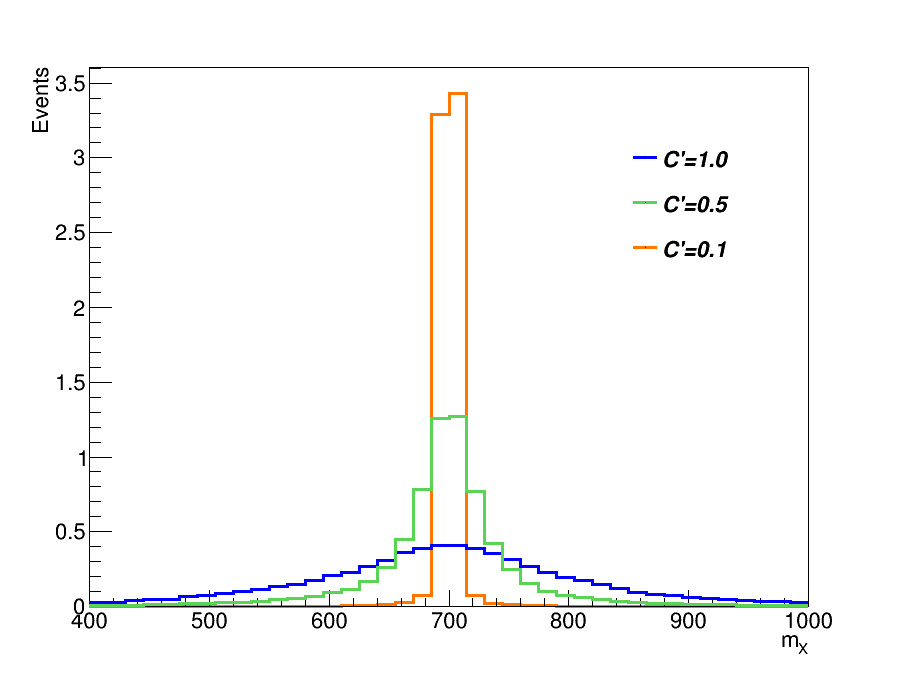
\includegraphics[width=0.45\textwidth]{../AN/Figs/higgsLHEmass700_cuts_nocuts.png}
}
\subfigure[$m_T^I$]{
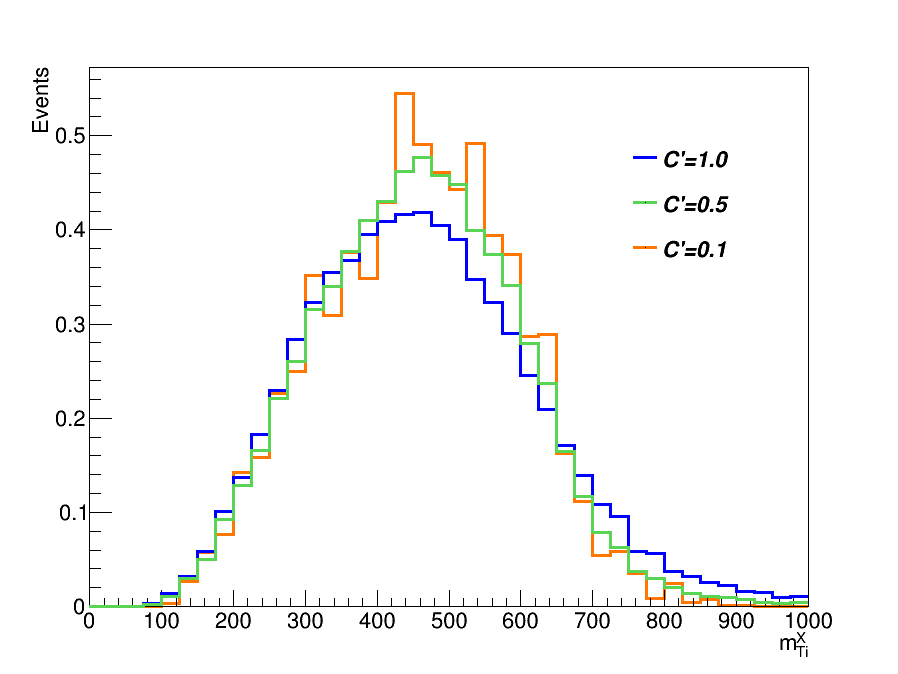
\includegraphics[width=0.45\textwidth]{../AN/Figs/mTi700_cuts_nocuts.png}
}
\caption{ Signal distributions at the MC generator level of $m_X$ and $m_T^I$ variables for different $C'$ values (1,0.5,0.1).}
    \label{fig:cprime}
\end{figure}

\subsection*{2HDM and MSSM models}
The 2HDM is a well motivated extension of the SM. It contains two Higgs doublets, from which a total of five Higgs bosons are predicted: 
two CP-even bosons $h$ and $H$, a CP-odd boson $A$ and two charged bosons $H^\pm$. In most theories, $h$ exhibits the features of the SM Higgs boson, while $H$ is a CP-even Higgs boson at a higher mass. The 2HDM comprises many free parameters. Two of these are of particular interest:
\begin{itemize}
\item $\tan\beta$: The ratio $\frac{v_u}{v_d}$ of the vacuum expectation values of the two Higgs doublets.
\item $\alpha$: The mixing angle of the two scalar Higgs bosons $h$ and $H$.
\end{itemize}
The quantity $\cos(\beta-\alpha)$ is also of interest, as the coupling of the heavy scalar Higgs boson $H$ to two vector bosons is proportional to this factor. In the decoupling limit, which occurs at $\cos(\beta-\alpha)=0$, all couplings become SM-like.
A 2HDM of type-2 is considered in this study. Here up-type quarks couple to one doublet, while down-type quarks and leptons couple to the other doublet.\\ 
\newline
%The MSSM is a type-2 2HDM. On tree level only two parameters are left free. By convention, these parameters are chosen to be $\tan\beta$ and $m_{A}$, the mass of the pseudoscalar Higgs boson. The exclusion limits can be set in a two-dimensional plane as a function of these two parameters. Due to higher order diagrams additional free parameters occur. Benchmark scenarios are then used in order to constrain these parameters. Here two MSSM scenarios are used: the $m_{h}^{mod+}$ scenario and the hMSSM scenario \cite{Gori:2130983}.
The necessary model predictions for these scenarios are provided by the LHC Higgs Cross Section Working Group \cite{bsmhiggsxsecs}. 
For both MSSM scenarios the gluon-gluon fusion cross sections have been computed with SusHi (v.1.4.1)\cite{Harlander:2012pb}. These cross sections include NLO supersymmetric QCD corrections and NNLO QCD corrections for the top quark contribution in the effective theory of a heavy top quark, as well as electroweak effects by light quarks. The masses of the Higgs bosons, their mixing, the branching fractions and the effective Yukawa couplings in the $m_{h}^{mod+}$ scenario are all calculated with FeynHiggs (v.2.10.2)\cite{Heinemeyer:1998yj, Heinemeyer:1998np, Degrassi:2002fi, Frank:2006yh, Hahn:2013ria}. For the hMSSM scenario the branching fractions are obtained from HDECAY (v.6.40)\cite{Djouadi:1997yw, Djouadi:2006bz}. The results for general 2HDM are obtained using the gluon-gluon fusion cross sections computed with SusHi (v.1.5.0) and the branching fractions from 2HDMC (v.1.7.0)\cite{Rathsman:2011yv}. The VBF cross sections are calculated using the following approximation: the BSM Higgs production cross sections for VBF, which are also provided by the LHC Higgs Cross Section Working Group \cite{bsmhiggsxsecs2}, are multiplied by $\cos^{2}(\beta-\alpha)$ to obtain the VBF cross sections for a heavy CP-even Higgs boson.\newline
The exclusion limits obtained for the MSSM scenarios are displayed in the $m_{A}$ vs $\tan\beta$ plane. A fine grid is chosen in this plane, and for each point of this grid a maximum likelihood fit is performed after the $m_{A}$ and/or $\tan\beta$ dependent values of the model, such as cross sections and masses of the Higgs bosons are calculated. 
%These fits are done using the asymptotic method. Performing a maximum likelihood fit in this manner is equivalent to a hypothesis test, where the signal hypothesis is tested against the SM and background hypothesis. 
The signal hypothesis for a combination of $m_{A}$ and $\tan\beta$ is excluded at $95\%$ confidence level. In the two-dimensional plane this limit is determined from interpolation between the points of the grid. The limits in the more general 2HDM are obtained in the same way, although a different parameter is chosen in place of $m_{A}$.



\section{Fully leptonic results}
\subsection*{Electroweak singlet sector}
No evidence for an excess of events with respect to the SM predictions  is observed and thus, exclusion
limits in the product of the cross section production times the BR of the decay to two W bosons is evaluated for the EW singlet model. The fraction of signal production via the VBF mechanism is fixed to the SM value.
The final binned fit is performed using the $m_T^I$ histogram for all signals and the number of events for the backgrounds for every mass point from
200\GeV up to 3\TeV and the 95\% CL upper exclusion limits are calculated. \\
\newline
In the fully leptonic analysis, a combination among the opposite flavour and same flavour analysis is performed. 
The expected and observed limit is shown in Fig.~\ref{fig:lim_OFSF_comb}. 
This analysis excludes the existence of a resonance in the mass range between 200 GeV and $\sim$2.5 TeV: 
the predicted high mass cross section (the red line in Fig.~\ref{fig:lim_OFSF_comb} is above the observed data in this mass range.
This limit represent a considerable improvement respect to the high mass search done with 2015 data, Fig.~\ref{lim_2015} 
and the expected and observed limits are also better with respect to the ATLAS results for the similar analysis, Fig.~\ref{ATLAS-CONF-2016-074_fig}.\\
\begin{figure}[htb]
\centering
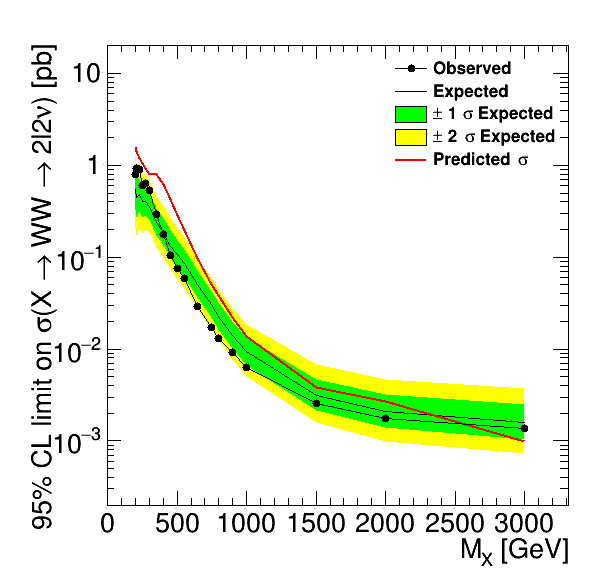
\includegraphics[width=0.75\textwidth]{../AN/Figs/unblinding/Limits/c2_FullComb_unbl.png}
\caption{Fully leptonic  exclusion limits at 95$\%$ CL on the cross section (gluon gluon fusion and VBF) times branching ration in $WW \to 2\ell 2\nu$ 
as a function of the mass. The red line represent the predicted cross-section for EW high mass bosons.}
\label{fig:lim_OFSF_comb}
\end{figure}



\subsection*{MSSM sector}
The exclusion limits are also extended to the MSSM model interpretation in terms of $m_A$.
The exclusion limits  for the $m_h^{mod+}$ scenario and for the hMSSM scenario are reported for the fully leptonic final state in Fig.~\ref{fig:MSSM}. 
The dashed line marks the expected limit, while the azure area shows  excluded limit obtained with the data. 
The bands in gray and dark gray surrounding the limit indicate the $\pm 1,2\sigma$ contours, 	respectively. 
For both scenarios the region at low values of $m_{A}$  (approximately $<150$ GeV) and low $\tan \beta$ value (approximately $<$20) are excluded. 
These results complement well with the exclusion limit given by the MSSM $H\rightarrow\tau\tau$ analysis, where the sensitivity is lower for low $m_{A}$ masses 
and low $\tan\beta$ values~\cite{CMS:2017epy}.\\
\newline
The exclusion limits for a 2HDM model are also evaluated.
In particular, the 2HDM limits for both the type-1 and the type-2 models are displayed in a $\cos(\beta-\alpha)$-$\tan\beta$ plane,  Fig.~\ref{fig:2HDMa}, 
in which the masses of neutral heavy Higgs  are $m_{H}=m_{A}=200$, $300$, $500$ GeV and the convention $\sin(\beta-\alpha) > 0$ is used. 
Instead  the limit in the  $m_{H}$-$\tan\beta$ plane are shown in Fig. ~\ref{fig:2HDMb}. 
Here it is again assumed that $m_{H}=m_{A}$ and $\sin(\beta-\alpha) > 0$, but here the relationship between $\beta$ and $\alpha$ is $\cos(\beta-\alpha)=0.1$. 
\begin{figure}[H]
\centering
\subfigure[$m_h^{mod+}$]{
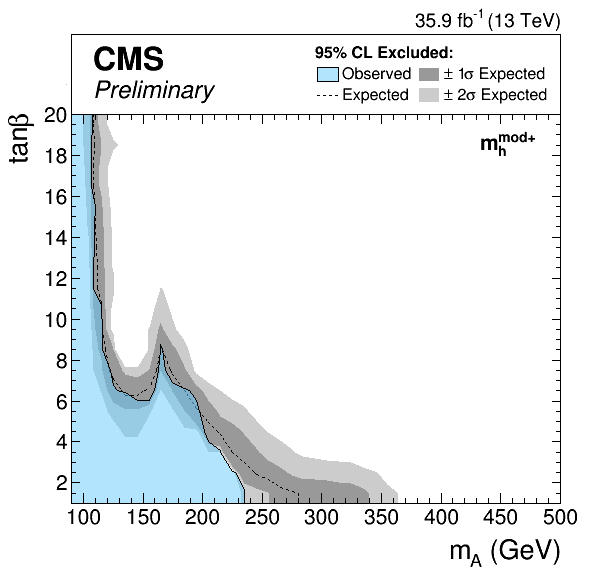
\includegraphics[width=0.45\textwidth]{../AN/Figs/unblinding/2HDM/mhmodp.png}
}
\subfigure[hMSSM]{
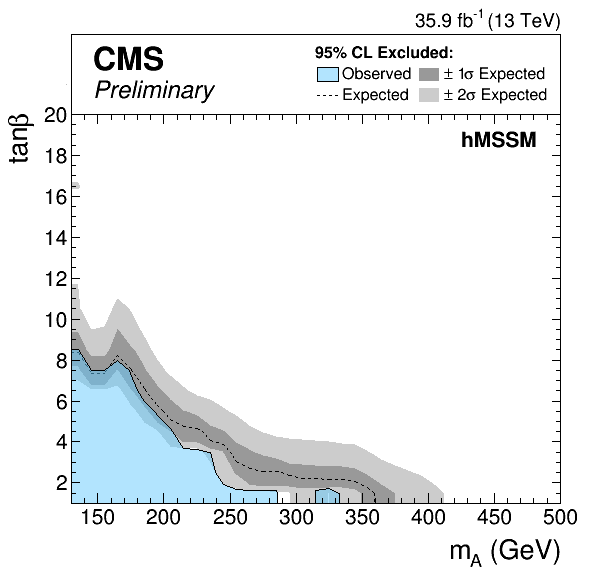
\includegraphics[width=0.45\textwidth]{../AN/Figs/unblinding/2HDM/hmssm.png}
}
\caption{(a) 95$\%$ CL exclusion limits for the MSSM $m_h^{mod+}$ scenario (b) for the hMSSM scenario.}
    \label{fig:MSSM}
\end{figure}



\begin{figure}[H]
\centering
\subfigure[Type-1, $m_{H}=200\,$GeV]{
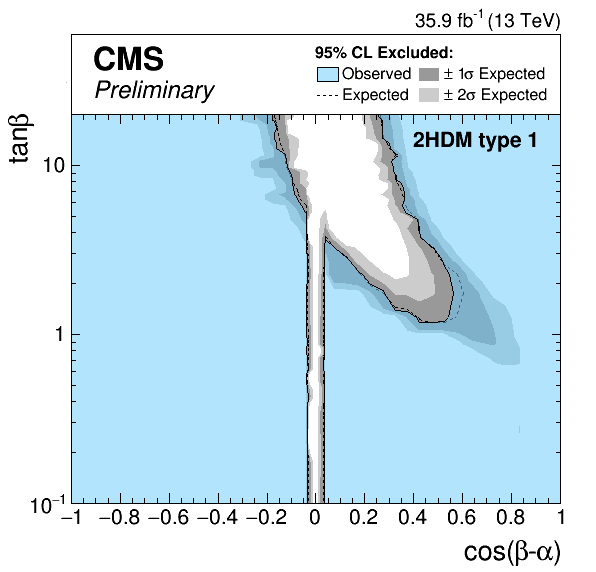
\includegraphics[width=0.45\textwidth]{../AN/Figs/unblinding/2HDM/thdm_cosba_t1_200.png}
}
\subfigure[Type-2, $m_{H}=200\,$GeV]{
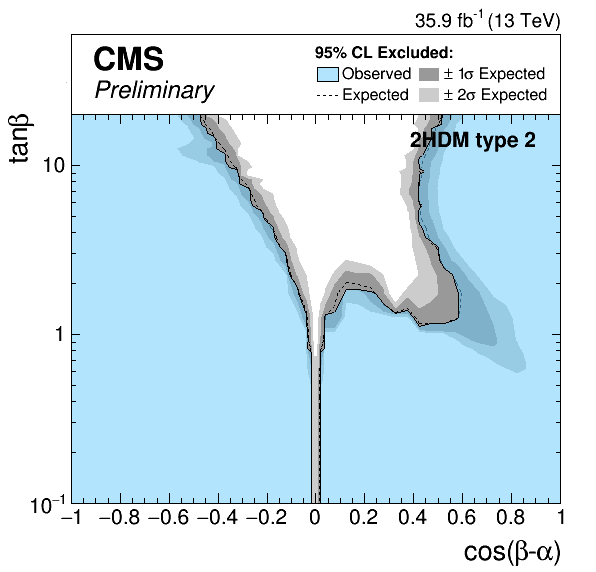
\includegraphics[width=0.45\textwidth]{../AN/Figs/unblinding/2HDM/thdm_cosba_t2_200.png}
}
\\
\subfigure[Type-1, $m_{H}=300\,$GeV]{
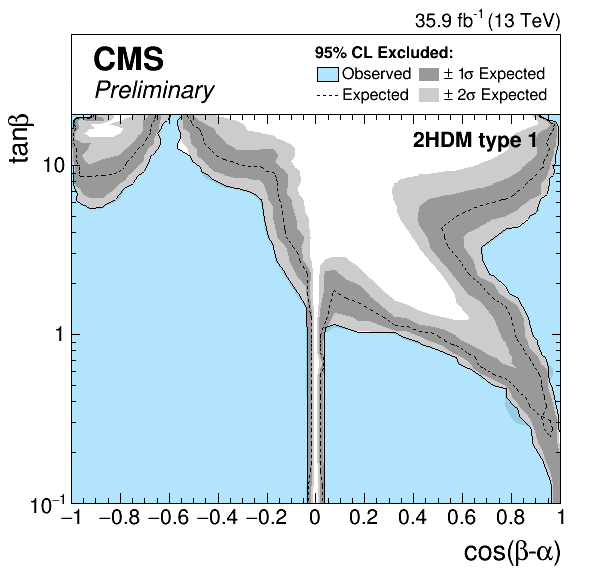
\includegraphics[width=0.45\textwidth]{../AN/Figs/unblinding/2HDM/thdm_cosba_t1_300.png}
}
\subfigure[Type-2, $m_{H}=300\,$GeV]{
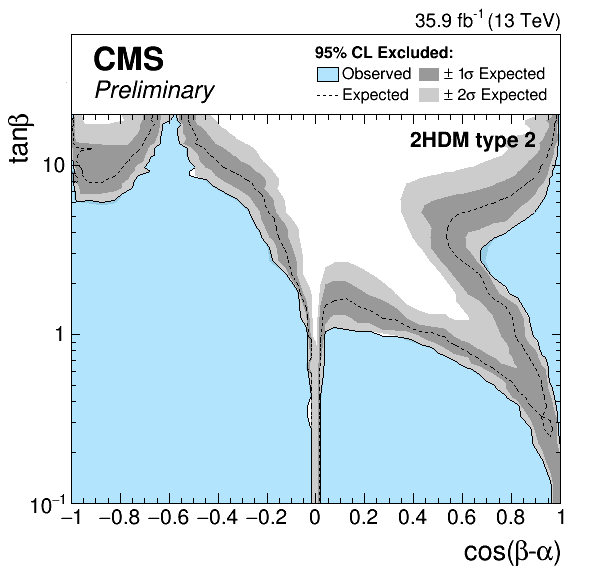
\includegraphics[width=0.45\textwidth]{../AN/Figs/unblinding/2HDM/thdm_cosba_t2_300.png}
}
\\
\subfigure[Type-1, $m_{H}=500\,$GeV]{
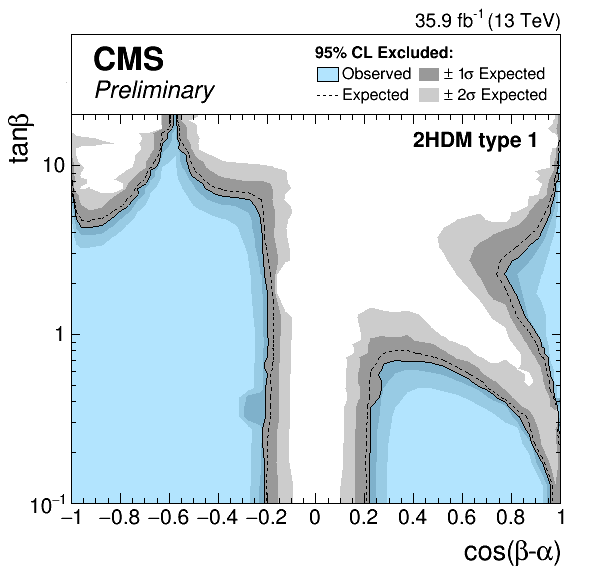
\includegraphics[width=0.45\textwidth]{../AN/Figs/unblinding/2HDM/thdm_cosba_t1_500.png}
}
\subfigure[Type-2, $m_{H}=500\,$GeV]{
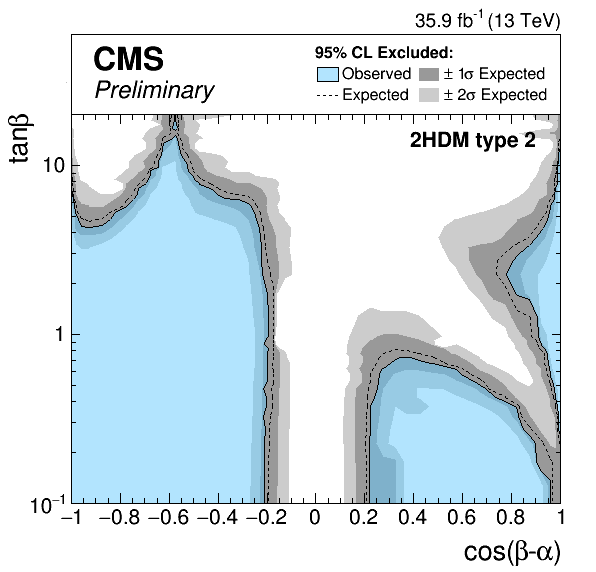
\includegraphics[width=0.45\textwidth]{../AN/Figs/unblinding/2HDM/thdm_cosba_t2_500.png}
}

\caption{95$\%$ CL exclusion limits on a 2HDM versus $\cos(\beta-\alpha)$. Limits are shown for a type-1 and type-2 2HDM for different masses $m_{H}=200$, $300$, $500\,$GeV.}
    \label{fig:2HDMa}
\end{figure}

\begin{figure}[H]
\centering
\subfigure[Type-1, $\cos(\beta-\alpha)=0.1$]{
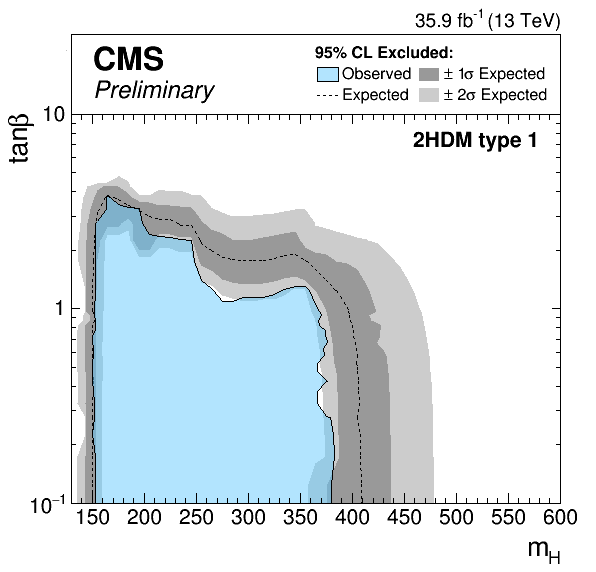
\includegraphics[width=0.45\textwidth]{../AN/Figs/unblinding/2HDM/thdm_mh_t1.png}
}
\subfigure[Type-2, $\cos(\beta-\alpha)=0.1$]{
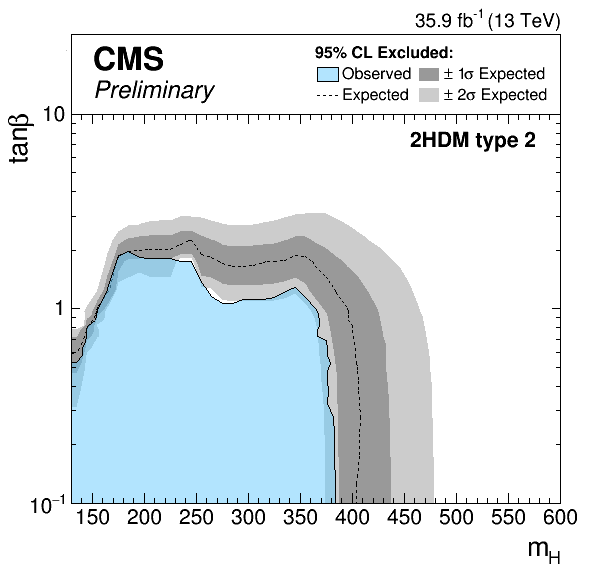
\includegraphics[width=0.45\textwidth]{../AN/Figs/unblinding/2HDM/thdm_mh_t2.png}
}

\caption{95$\%$ CL exclusion limits on a 2HDM versus $m_{H}$. Limits are shown for a type-1 and type-2 2HDM for $\cos(\beta-\alpha)=0.1$.}
    \label{fig:2HDMb}
\end{figure}


\section{Combination among the fully and the semileptonic analysis}
The same procedure described for the fully leptonic analysis is also adopted to evaluate the cross section limits 
for the EW model interpretation using the semileptonic final state, Fig~\ref{limit_observed_lnuqq_VBF0_log-1}.
\begin{figure}[htb]
\centering
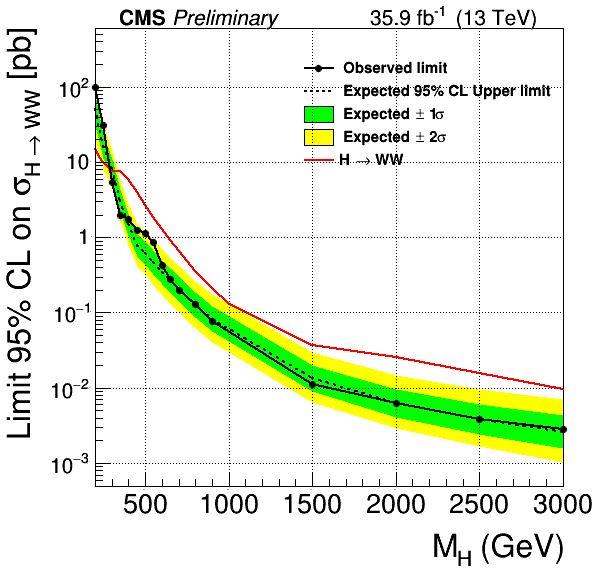
\includegraphics[width=0.65\textwidth]{../Cap6/lnuqq}
\caption{Semileptonic exclusion limits at 95$\%$ CL  on the production cross section (gluon gluon fusion and VBF) times branching ration in $WW$ as a function of the mass.  The red line represent the predicted cross-section for EW high mass bosons.}
\label{limit_observed_lnuqq_VBF0_log-1}
\end{figure}
It is evident that the fully and semileptonic analysis are complementary: 
the former sets a powerful limit at low mass ($<$ 1 TeV), the other at  high mass\footnote{To correctly compare Fig.~\ref{fig:lim_OFSF_comb} with  Fig~\ref{limit_observed_lnuqq_VBF0_log-1}, the limits for the 
fully leptonic channel must be multiplied by a factor of $\sim$10 to take in account the BR of the W's in $ 2\ell 2\nu$.\\
}. For this reason a combination among the two analysis is desirable.
\newline
The  combination of the fully leptonic and semileptonic analysis has been performed and the limits are shown in Fig.~\ref{lim_superC}. 
The values of the upper limits are comparable with the results obtained by CMS in $X \to ZZ$ with final state ($4\ell$, $2\ell 2\nu$ and $2\ell 2q$) \cite{Sirunyan:2018qlb} and represent a very tight constraint on the existence of  high mass particle: 
they are among the most stringent exclusion limits obtained by any LHC experiments.\\
\newline
For these results the fraction of the $X$ resonance production via VBF  ($f_{VBF}$)  was fixed to the SM fraction. 
However by performing a scan of the fraction $f_{VBF}$ it is possible to evaluate the upper limits in different scenarios. 
Given this fraction, $\sigma_X \times f_{VBF}$ represents the VBF  cross-section, while
the gluon-gluon fusion cross-section is $\sigma_X \times ( 1-  f_{VBF} )$. 
Three different values of  $f_{VBF}$ are studied:   $f_{VBF}$ free to floating, $f_{VBF}=$ 0 and $f_{VBF}=$ 1. 
The upper limits for three cases are shown in Fig.~\ref{wwe}  for the combination of the fully and same leptonic analysis.
\begin{figure}[H]
\centering
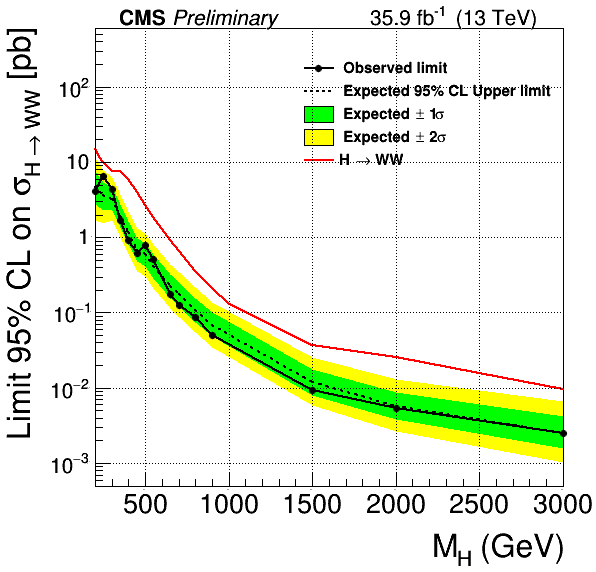
\includegraphics[width=0.65\textwidth]{../Cap6/all}
\caption{Expected and observed exclusion limits at 95\% CL on the sum of gluon-gluon fusion and VBF cross
sections times branching fraction for the combination of all the analysis categories as a function
of the resonance mass. The black dotted line corresponds to the central expected value while
the yellow and green bands represent the $\pm 1 \sigma$ and $\pm 2 \sigma$ uncertainties respectively.}
\label{lim_superC}
\end{figure}
\begin{figure}[htb]
\centering
\subfigure[ $f_{VBF}=$ free to float ]{
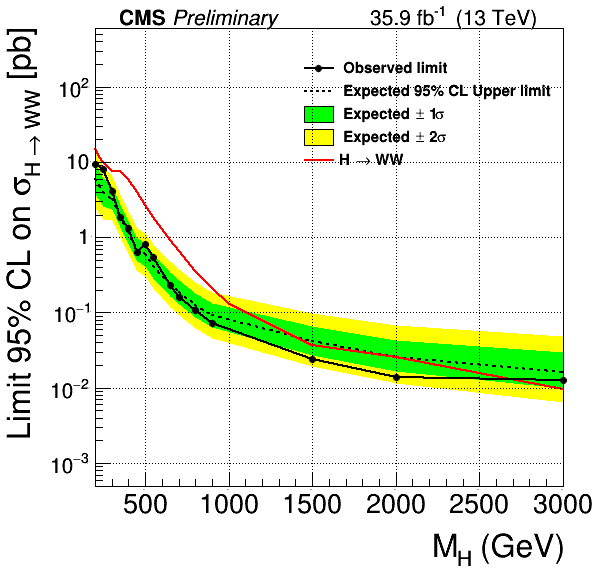
\includegraphics[width=0.45\textwidth]{../Cap6/vbfX}
}
\subfigure[ $f_{VBF}=$0 ]{
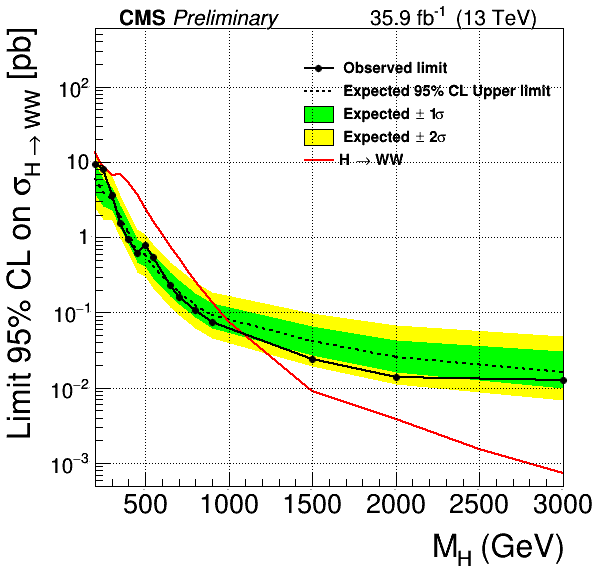
\includegraphics[width=0.45\textwidth]{../Cap6/vbf0}
}
\subfigure[ $f_{VBF}=$ 1]{
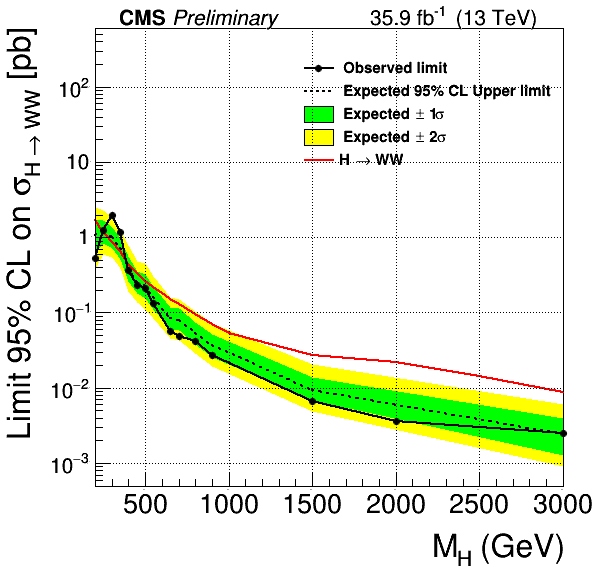
\includegraphics[width=0.45\textwidth]{../Cap6/vbf1}
}
\caption{95\% CL exclusion limits, on the production gluon-gluon fusion and VBF cross section times branching 
for different $f_{VBF}$ fraction. The red line represent the predicted cross-section for EW high
mass bosons in the free floating case (a), only the predicted vector boson cross-section in
 $f_{VBF}$ case (b) and only the predicted gluon-gluon fusion cross-section in $f_{VBF}$ case (c).}
    \label{wwe}
\end{figure}
The MSSM limits  as a function of $m_A$ are computed for the combination among the two analysis, Fig.~\ref{fig:MSSM2}.
Finally the limits interpretation in terms of 2HDM type-I and type-II are evaluated and the results is show in Fig.\ref{fig:2HDM1} and Fig.\ref{fig:2HDM2}
Comparing the fully leptonic and combination it is clear that the main part of the exclusion limits are given by the fully leptonic analysis 	
although with the contribution of semileptonic they are further improved.
\begin{figure}[htb]
\centering
\subfigure[$m_h^{mod+}$]{
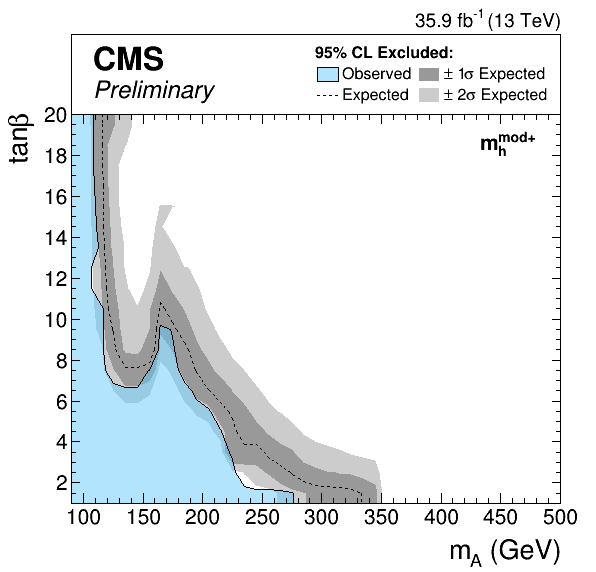
\includegraphics[width=0.45\textwidth]{../Cap6/mhmodp}
}
\subfigure[hMSSM]{
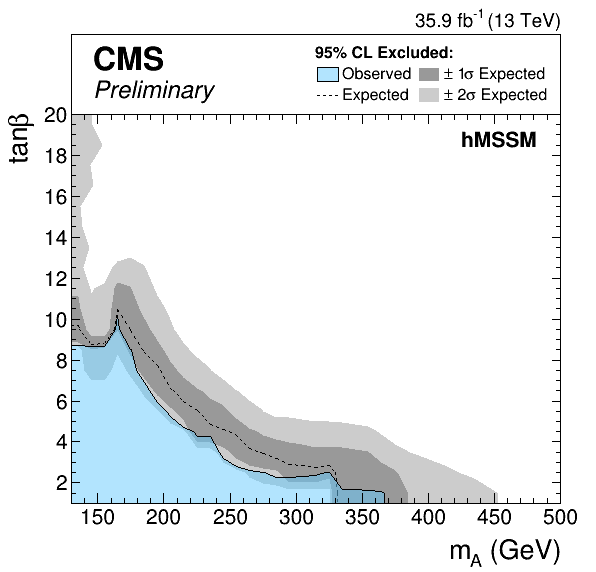
\includegraphics[width=0.45\textwidth]{../Cap6/hmssm}
}
\caption{(a) 95$\%$ CL exclusion limits for the MSSM $m_h^{mod+}$ scenario (b) for the hMSSM scenario.}
    \label{fig:MSSM2}
\end{figure}


\begin{figure}[htb]
\centering
\subfigure[Type-1, $m_{H}=200\,$GeV]{
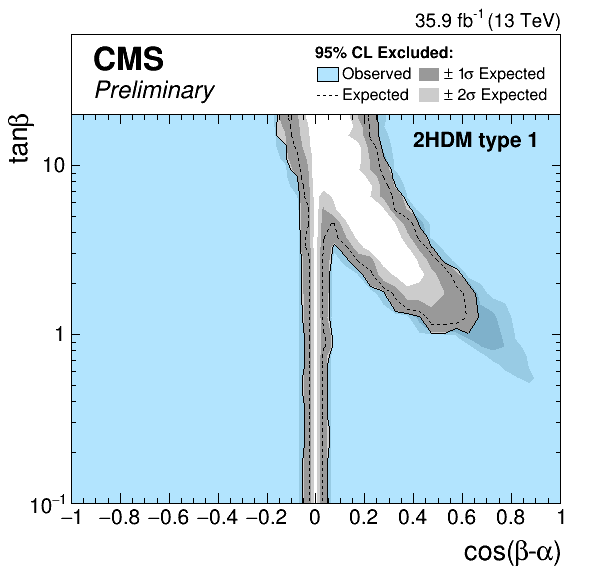
\includegraphics[width=0.45\textwidth]{../Cap6/thdm_cosba_t1_200.png}
}
\subfigure[Type-2, $m_{H}=200\,$GeV]{
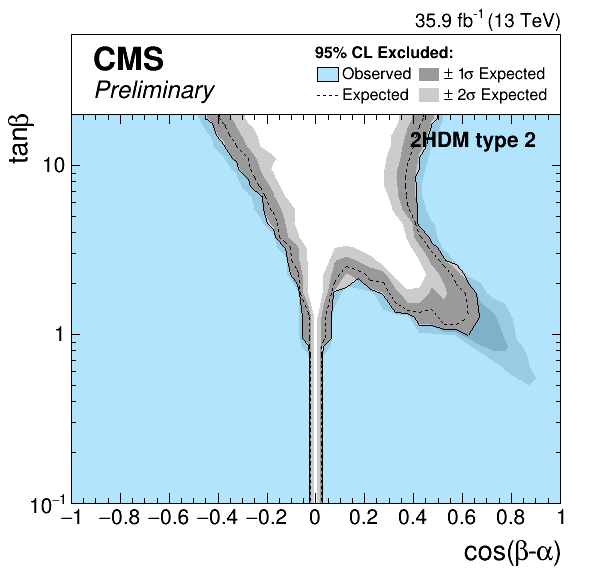
\includegraphics[width=0.45\textwidth]{../Cap6/thdm_cosba_t2_200.png}
}
\\
\subfigure[Type-1, $m_{H}=300\,$GeV]{
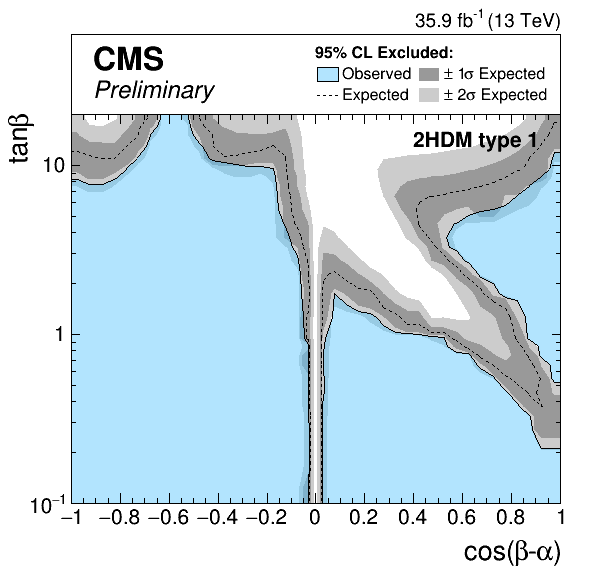
\includegraphics[width=0.45\textwidth]{../Cap6/thdm_cosba_t1_300.png}
}
\subfigure[Type-2, $m_{H}=300\,$GeV]{
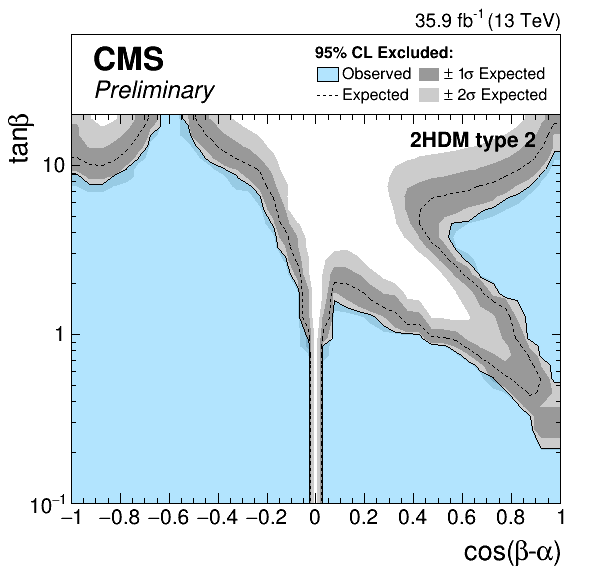
\includegraphics[width=0.45\textwidth]{../Cap6/thdm_cosba_t2_300.png}
}
\\
\subfigure[Type-1, $m_{H}=500\,$GeV]{
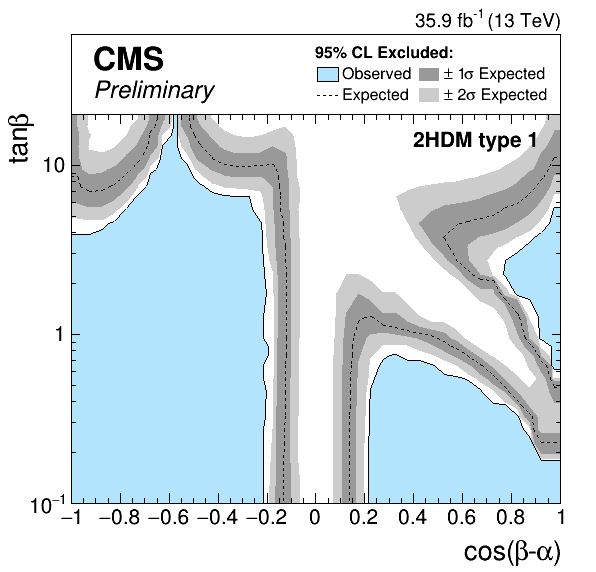
\includegraphics[width=0.45\textwidth]{../Cap6/thdm_cosba_t1_500.png}
}
\subfigure[Type-2, $m_{H}=500\,$GeV]{
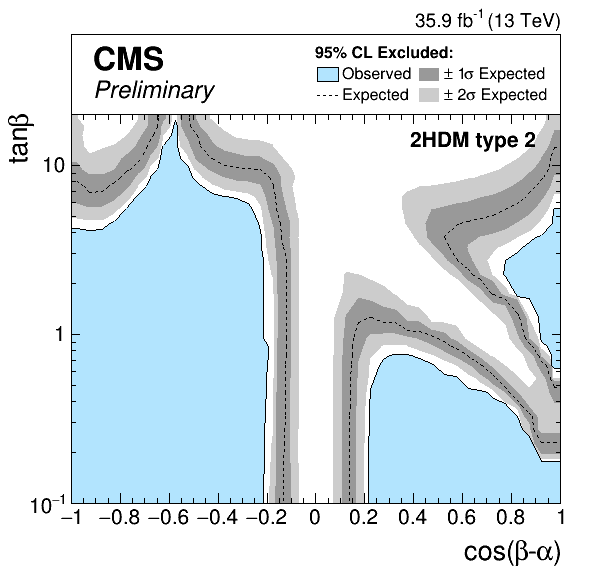
\includegraphics[width=0.45\textwidth]{../Cap6/thdm_cosba_t2_500.png}
}
\caption{95$\%$ CL exclusion limits on a 2HDM versus $\cos(\beta-\alpha)$. Limits are shown for a type-1 and type-2 2HDM for different masses $m_{H}=200$, $300$, $500\,$GeV.}
    \label{fig:2HDM1}
\end{figure}

\begin{figure}[htb]
\centering
\subfigure[Type-1, $\cos(\beta-\alpha)=0.1$]{
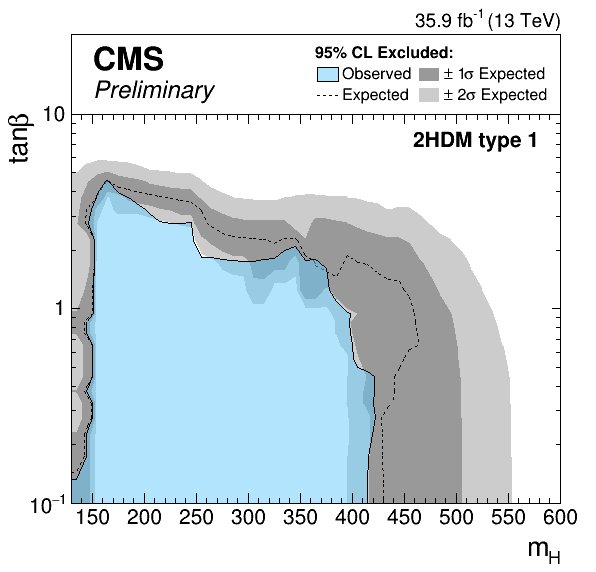
\includegraphics[width=0.45\textwidth]{../Cap6/thdm_mhtanb_t1}
}
\subfigure[Type-2, $\cos(\beta-\alpha)=0.1$]{
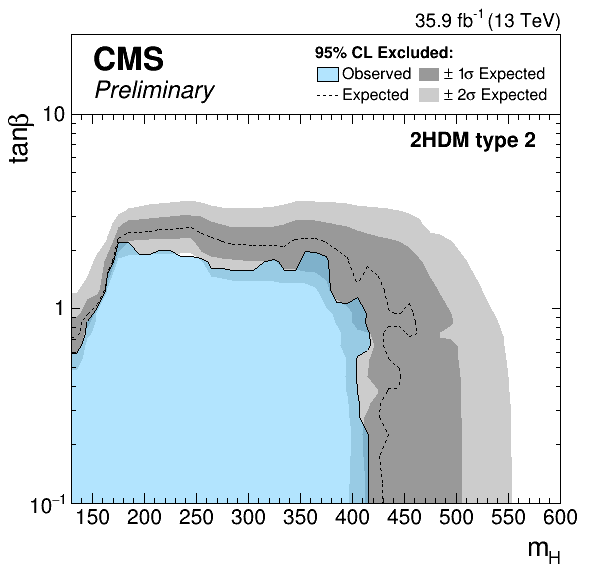
\includegraphics[width=0.45\textwidth]{../Cap6/thdm_mhtanb_t2}
}

\caption{95$\%$ CL exclusion limits on a 2HDM versus $m_{H}$. Limits are shown for a type-1 and type-2 2HDM for $\cos(\beta-\alpha)=0.1$.}
    \label{fig:2HDM2}
\end{figure}



\chapter*{Conclusion}
A search for a Higgs-like boson in $X \to \ W^+W^-$ with fully leptonic and semileptonic final state, produced via gluon-gluon fusion and VBF 
mechanism, has been performed in the mass range between 200 GeV and 3 TeV.
Data collected by the CMS experiment during 2016 at $\sqrt{s}=13$ TeV, for a total luminosity of $35.9$ fb$^{-1}$, have been used.
This channel has a high branching ratio but a full reconstruction of the final state is not possible due to the presence of neutrinos. 
The main sources of background in this channel are represented by WW, Drell-Yan, Top, W+jet and multiboson.
Different kinematic cuts are applied, in order to tag the fully or semileptonic final states and reduce background. 
To increase the sensitivity to a scalar resonance, events are categorized according to the final state, the number of jets 
and the jet kinematics. 
The final statistical analysis is a template analysis performed on the ``improved transverse mass'', a dedicate variable
introduced for this specific analysis. 
The interference between the high mass signal, the WW background and the SM Higgs boson has been studied for both the gluon-gluon fusion and the VBF mechanism production.
This contribution is not negligible, especially for high mass values, so it has been included in the template for the signal.\\
\newline
The result of the analysis is that no signal excess is observed in the distribution of the reconstructed $m_T^I$ variable of the $X$ candidate.
Two BSM models are investigated in order to set limits: the Electroweak singlet and the Two Higgs Doublet Model. 
In the Electroweak singlet model, exclusion limits have been set at 95\% CL on the production cross section of a scalar neutral boson
in the mass range from 200 GeV to 3 TeV.
These limits represent a considerable enhancement with respect the past analyses 
targeting the same fine state in the ATLAS and CMS experiments.
In the context of MSSM and  2HDM type-I and type-II scenarios, exclusion limits are set in the parameter space ($M_A$, $\tan \beta$) for the MSSM, and ($\cos(\alpha - \beta)$, $\tan \beta$) for generic
2HDM. Compared to other searches performed at the LHC, the excluded regions set new relevant constraints for both scenarios.\\
\newline
Due to its high discovery potential, this high mass search is recognized as a key analysis of the LHC and HL-LHC physics
program. In future, with the full Run II data it will be possible to expand the mass range
of this search further and set even tighter limits on the production cross section of a new Higgs-like resonance.












